% Source: StudentGovernmentRepo/Common_Sense_Carolina_Lobbying_org/figures/org_phase6.tex
\documentclass[border=15pt]{standalone}
\usepackage{tikz}
\usepackage{xcolor}
\usetikzlibrary{positioning, arrows.meta, calc, fit, backgrounds}
\definecolor{garnet}{HTML}{73000A}
\definecolor{lightgarnet}{HTML}{F5EAEB}
\definecolor{sandstorm}{HTML}{FFF2E3}
\definecolor{rose}{HTML}{CC2E40}
\definecolor{atlantic}{HTML}{466A9F}
\definecolor{congaree}{HTML}{1F414D}
\definecolor{horseshoe}{HTML}{65780B}
\definecolor{honeycomb}{HTML}{A49137}
\definecolor{grass}{HTML}{CED318}
\definecolor{warmgrey}{HTML}{676156}
\definecolor{tenblack}{HTML}{ECECEC}

\begin{document}
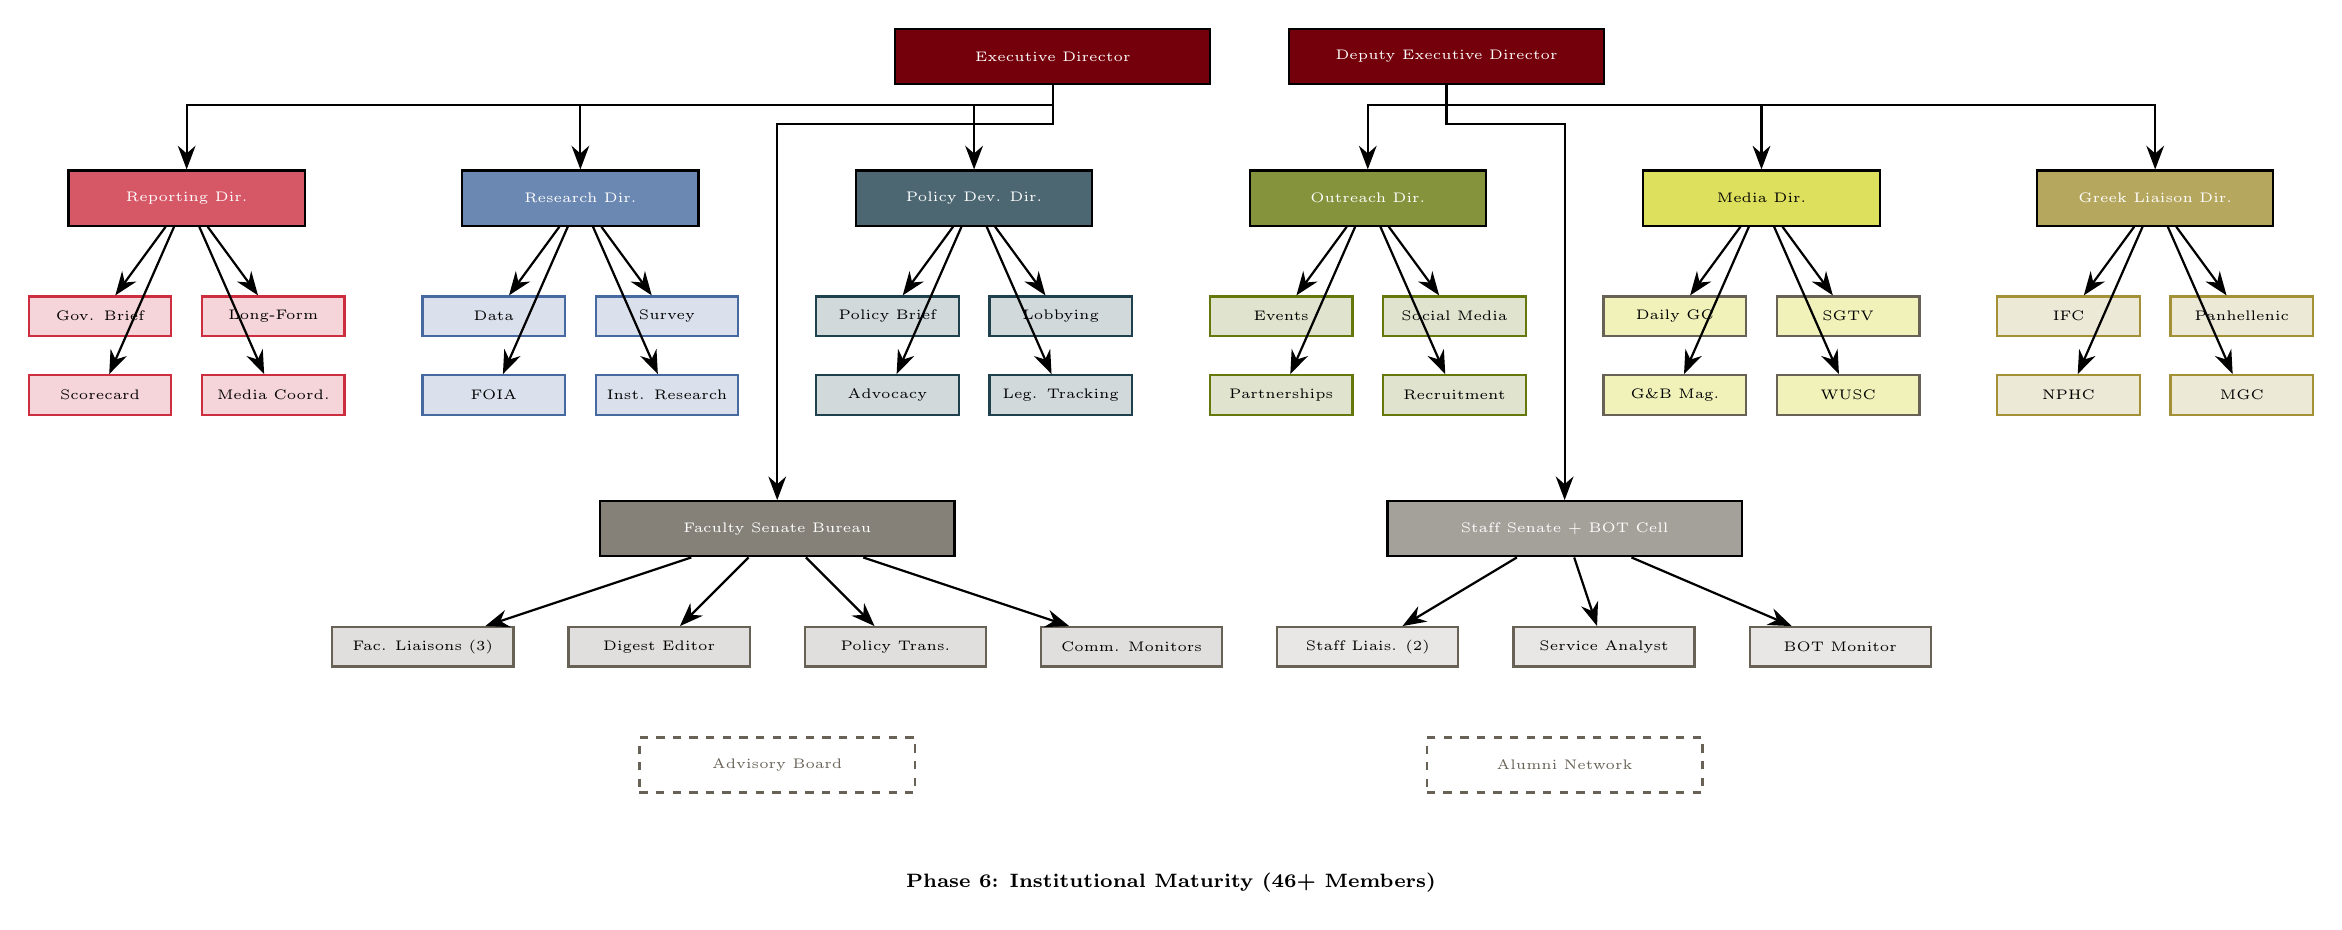
\begin{tikzpicture}[
  >=Stealth,
  thick,
  every node/.style={rectangle, draw, align=center, sharp corners, font=\tiny},
  arr/.style={-{Stealth[length=3mm]}, thick},
  %% Leaf node: text width=1.6cm forces wrapping, inner sep=3pt.
  %% Rendered width = 1.6cm + 2*0.1cm = ~1.8cm.
  leaf/.style={minimum height=0.5cm, inner sep=3pt, text width=1.6cm}
]

%% ─── Row 0: Executive tier (y=0) ────────────────────────────────────────────
\node[fill=garnet, text=white, minimum width=4cm, minimum height=0.7cm]
  (ed) at (-1.5,0) {Executive Director};

\node[fill=garnet, text=white, minimum width=4cm, minimum height=0.7cm]
  (ded) at (3.5,0) {Deputy Executive Director};

%% ─── Row 1: Directors (y=-1.8) ──────────────────────────────────────────────
%% 6 directors spaced 5cm apart, centered at 0
\node[fill=rose!80, text=white, minimum width=3cm, minimum height=0.7cm]
  (repdir) at (-12.5,-1.8) {Reporting Dir.};

\node[fill=atlantic!80, text=white, minimum width=3cm, minimum height=0.7cm]
  (resdir) at (-7.5,-1.8) {Research Dir.};

\node[fill=congaree!80, text=white, minimum width=3cm, minimum height=0.7cm]
  (poldir) at (-2.5,-1.8) {Policy Dev. Dir.};

\node[fill=horseshoe!80, text=white, minimum width=3cm, minimum height=0.7cm]
  (outdir) at (2.5,-1.8) {Outreach Dir.};

\node[fill=grass!70, text=black, minimum width=3cm, minimum height=0.7cm]
  (meddir) at (7.5,-1.8) {Media Dir.};

\node[fill=honeycomb!80, text=white, minimum width=3cm, minimum height=0.7cm]
  (grkdir) at (12.5,-1.8) {Greek Liaison Dir.};

%% Row 0 to Row 1 arrows
\draw[arr] (ed.south)  -- ++(0,-0.25) -| (repdir.north);
\draw[arr] (ed.south)  -- ++(0,-0.25) -| (resdir.north);
\draw[arr] (ed.south)  -- ++(0,-0.25) -| (poldir.north);
\draw[arr] (ded.south) -- ++(0,-0.25) -| (outdir.north);
\draw[arr] (ded.south) -- ++(0,-0.25) -| (meddir.north);
\draw[arr] (ded.south) -- ++(0,-0.25) -| (grkdir.north);

%% ─── Rows 2-3: Sub-units in 2x2 grids per director ─────────────────────────
%% Each director has 4 sub-nodes: 2 at y=-3.3, 2 at y=-4.3.
%% Within each row: centers at dir_x -1.1 and dir_x +1.1 (2.2cm apart).
%% Between adjacent directors: 5.0 - 1.1 = 3.9cm gap (safe with 1.8cm nodes).

%% Under Reporting Dir. (x=-12.5)
\node[leaf, fill=rose!20, draw=rose]
  (r1) at (-13.6,-3.3) {Gov. Brief};
\node[leaf, fill=rose!20, draw=rose]
  (r2) at (-11.4,-3.3) {Long-Form};
\node[leaf, fill=rose!20, draw=rose]
  (r3) at (-13.6,-4.3) {Scorecard};
\node[leaf, fill=rose!20, draw=rose]
  (r4) at (-11.4,-4.3) {Media Coord.};

\draw[arr] (repdir) -- (r1);
\draw[arr] (repdir) -- (r2);
\draw[arr] (repdir) -- (r3);
\draw[arr] (repdir) -- (r4);

%% Under Research Dir. (x=-7.5)
\node[leaf, fill=atlantic!20, draw=atlantic]
  (s1) at (-8.6,-3.3) {Data};
\node[leaf, fill=atlantic!20, draw=atlantic]
  (s2) at (-6.4,-3.3) {Survey};
\node[leaf, fill=atlantic!20, draw=atlantic]
  (s3) at (-8.6,-4.3) {FOIA};
\node[leaf, fill=atlantic!20, draw=atlantic]
  (s4) at (-6.4,-4.3) {Inst. Research};

\draw[arr] (resdir) -- (s1);
\draw[arr] (resdir) -- (s2);
\draw[arr] (resdir) -- (s3);
\draw[arr] (resdir) -- (s4);

%% Under Policy Dev. Dir. (x=-2.5)
\node[leaf, fill=congaree!20, draw=congaree]
  (p1) at (-3.6,-3.3) {Policy Brief};
\node[leaf, fill=congaree!20, draw=congaree]
  (p2) at (-1.4,-3.3) {Lobbying};
\node[leaf, fill=congaree!20, draw=congaree]
  (p3) at (-3.6,-4.3) {Advocacy};
\node[leaf, fill=congaree!20, draw=congaree]
  (p4) at (-1.4,-4.3) {Leg. Tracking};

\draw[arr] (poldir) -- (p1);
\draw[arr] (poldir) -- (p2);
\draw[arr] (poldir) -- (p3);
\draw[arr] (poldir) -- (p4);

%% Under Outreach Dir. (x=2.5)
\node[leaf, fill=horseshoe!20, draw=horseshoe]
  (o1) at (1.4,-3.3) {Events};
\node[leaf, fill=horseshoe!20, draw=horseshoe]
  (o2) at (3.6,-3.3) {Social Media};
\node[leaf, fill=horseshoe!20, draw=horseshoe]
  (o3) at (1.4,-4.3) {Partnerships};
\node[leaf, fill=horseshoe!20, draw=horseshoe]
  (o4) at (3.6,-4.3) {Recruitment};

\draw[arr] (outdir) -- (o1);
\draw[arr] (outdir) -- (o2);
\draw[arr] (outdir) -- (o3);
\draw[arr] (outdir) -- (o4);

%% Under Media Dir. (x=7.5)
\node[leaf, fill=grass!30, draw=warmgrey]
  (m1) at (6.4,-3.3) {Daily GC};
\node[leaf, fill=grass!30, draw=warmgrey]
  (m2) at (8.6,-3.3) {SGTV};
\node[leaf, fill=grass!30, draw=warmgrey]
  (m3) at (6.4,-4.3) {G\&B Mag.};
\node[leaf, fill=grass!30, draw=warmgrey]
  (m4) at (8.6,-4.3) {WUSC};

\draw[arr] (meddir) -- (m1);
\draw[arr] (meddir) -- (m2);
\draw[arr] (meddir) -- (m3);
\draw[arr] (meddir) -- (m4);

%% Under Greek Liaison Dir. (x=12.5)
\node[leaf, fill=honeycomb!20, draw=honeycomb]
  (g1) at (11.4,-3.3) {IFC};
\node[leaf, fill=honeycomb!20, draw=honeycomb]
  (g2) at (13.6,-3.3) {Panhellenic};
\node[leaf, fill=honeycomb!20, draw=honeycomb]
  (g3) at (11.4,-4.3) {NPHC};
\node[leaf, fill=honeycomb!20, draw=honeycomb]
  (g4) at (13.6,-4.3) {MGC};

\draw[arr] (grkdir) -- (g1);
\draw[arr] (grkdir) -- (g2);
\draw[arr] (grkdir) -- (g3);
\draw[arr] (grkdir) -- (g4);

%% ─── Row 4: Faculty Senate Bureau (y=-6, x=-5) ─────────────────────────────
\node[fill=warmgrey!80, text=white, minimum width=4.5cm, minimum height=0.7cm]
  (fsbhdr) at (-5,-6) {Faculty Senate Bureau};

\draw[arr] (ed.south) -- ++(0,-0.5) -| (fsbhdr.north);

%% Faculty Bureau sub-items (y=-7.5)
%% 4 nodes, min width=2.3cm, spacing=3.0cm
\node[fill=warmgrey!20, draw=warmgrey, minimum width=2.3cm, minimum height=0.5cm]
  (fb1) at (-9.5,-7.5) {Fac. Liaisons (3)};
\node[fill=warmgrey!20, draw=warmgrey, minimum width=2.3cm, minimum height=0.5cm]
  (fb2) at (-6.5,-7.5) {Digest Editor};
\node[fill=warmgrey!20, draw=warmgrey, minimum width=2.3cm, minimum height=0.5cm]
  (fb3) at (-3.5,-7.5) {Policy Trans.};
\node[fill=warmgrey!20, draw=warmgrey, minimum width=2.3cm, minimum height=0.5cm]
  (fb4) at (-0.5,-7.5) {Comm. Monitors};

\draw[arr] (fsbhdr) -- (fb1);
\draw[arr] (fsbhdr) -- (fb2);
\draw[arr] (fsbhdr) -- (fb3);
\draw[arr] (fsbhdr) -- (fb4);

%% ─── Row 4: Staff Senate + BOT Cell (y=-6, x=5) ────────────────────────────
\node[fill=warmgrey!60, text=white, minimum width=4.5cm, minimum height=0.7cm]
  (sschdr) at (5,-6) {Staff Senate + BOT Cell};

\draw[arr] (ded.south) -- ++(0,-0.5) -| (sschdr.north);

%% Staff/BOT sub-items (y=-7.5)
\node[fill=warmgrey!15, draw=warmgrey, minimum width=2.3cm, minimum height=0.5cm]
  (sb1) at (2.5,-7.5) {Staff Liais. (2)};
\node[fill=warmgrey!15, draw=warmgrey, minimum width=2.3cm, minimum height=0.5cm]
  (sb2) at (5.5,-7.5) {Service Analyst};
\node[fill=warmgrey!15, draw=warmgrey, minimum width=2.3cm, minimum height=0.5cm]
  (sb3) at (8.5,-7.5) {BOT Monitor};

\draw[arr] (sschdr) -- (sb1);
\draw[arr] (sschdr) -- (sb2);
\draw[arr] (sschdr) -- (sb3);

%% ─── Bottom row (y=-9) ─────────────────────────────────────────────────────
\node[draw=warmgrey, dashed, fill=none, minimum width=3.5cm, minimum height=0.7cm,
      text=warmgrey] (advbd) at (-5,-9) {Advisory Board};

\node[draw=warmgrey, dashed, fill=none, minimum width=3.5cm, minimum height=0.7cm,
      text=warmgrey] (alum)  at (5,-9)  {Alumni Network};

%% ─── Title (y=-10.5) ──────────────────────────────────────────────────────────
\node[draw=none, fill=none, font=\scriptsize\bfseries] at (0,-10.5)
  {Phase 6: Institutional Maturity (46+ Members)};

\end{tikzpicture}
\end{document}
